%-----------------------------------------------------------------
%	MODELS
%	!TEX root = ./main.tex
%-----------------------------------------------------------------
\section{Controller Implementation}

%-------------------------------
\subsection{Open-Loop Response}
\begin{frame}[fragile]{Open-Loop Response: Implementation}

\begin{lstlisting}[language=mymatlab]
% Time in seconds
t = 0:0.01:10;
% Input
u = zeros(size(t))*r;
% Create state space object
sys = ss(A,B,C,0);

% Calculate open-loop response
[y,t,x] = lsim(sys,u,t,phi_0);
\end{lstlisting}

\begin{itemize}
    \item \inline{ss()} defines the state space.
    \item \inline{lsim()} simulates the output time response $y(t)$ of dynamic system with input $u(t)$.
\end{itemize}
\end{frame}

\begin{frame}{Open-Loop Response: Simulation}
\begin{onlyenv}<1>
    \begin{figure}[H]
    	\centering
    	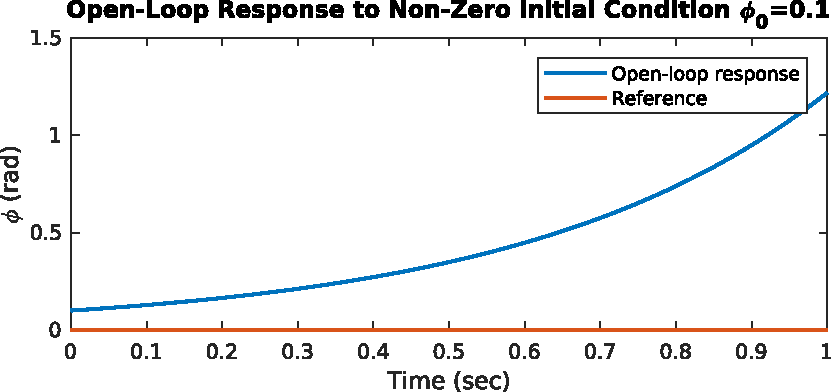
\includegraphics[width=0.7\textwidth]{images/curve-open-loop}
    	\caption{Open-Loop response to non-zero initial condition driving backwards with a trailer}
    	\label{fig:curve-open-loop}
    \end{figure}
\end{onlyenv}

\begin{onlyenv}<2>
    \begin{figure}[H]
    	\centering
    	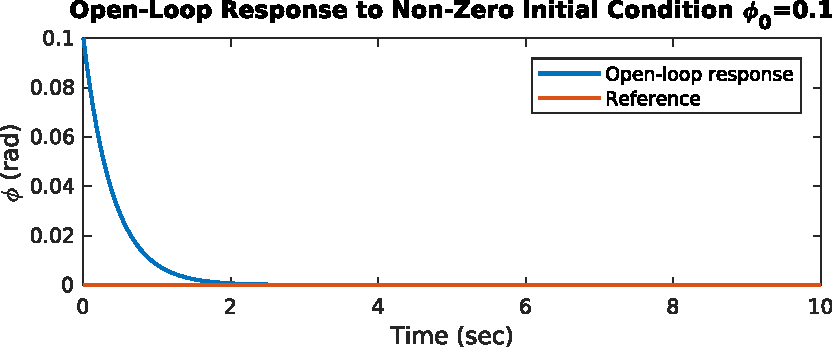
\includegraphics[width=0.73\textwidth]{images/stable-open-loop}
    	\caption{Open-Loop response to non-zero initial condition driving forwards with a trailer}
    	\label{fig:curve-open-loop-stable}
    \end{figure}
\end{onlyenv}
\end{frame}

%-------------------------------
\subsection{Closed-Loop Response}
\begin{frame}[fragile]{Closed-Loop Response: Implementation}

\begin{lstlisting}[language=mymatlab]
% Time in seconds
t = 0:0.01:60;
% Inputs
u = curve4(t, 0.4); % S shape
% Apply pole placement
K = place(A,B,-0.73);
% State space
sys_cl = ss(A-B*K,B,C,0);
% Calculate scaling factor
Nbar = rscale(sys,K);

% Calculate closed-loop response
[y_cl,t,x_cl] = lsim(sys_cl,Nbar*u,t,phi_0);
\end{lstlisting}

\begin{itemize}
    \item \inline{place()} finds the state-feedback gain $K$ and provides the desired closed-loop pole.
    \item \inline{rscale()} computes the desired scale factor $\bar{N}$.
\end{itemize}
\end{frame}

\begin{frame}{Closed-Loop Response: Simulation}
\begin{figure}[H]
	\centering
	\subfloat[Diagram of the curve]{%
		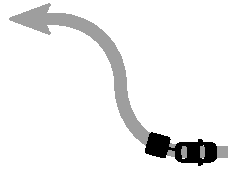
\includegraphics[height=0.15\textwidth]{images/curve4-diagram}%
		\label{fig:curve4a}%
		}%
	\hspace{0.5cm}%
	\subfloat[Closed-loop response of the controller]{%
		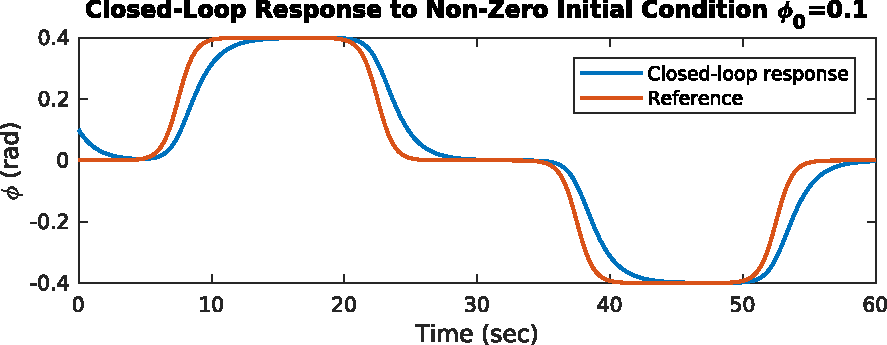
\includegraphics[height=0.28\textwidth]{images/control4-plot}%
		\label{fig:curve4b}%
		}%
	\caption{Diagram and control of the car-trailer system in a $S$-shaped curve}
\end{figure}

\footnotesize{Available at \url{https://github.com/aldomann/trailer-parking}}

\end{frame}

% \begin{frame}{Video test}
% 	\movie[width=10cm,height=6cm,poster]{Video}{videos/test.mp4}
% \end{frame}
